\documentclass[aspectratio=169,11pt]{beamer}

\usetheme{default}
\setbeamertemplate{navigation symbols}{}
\setbeamertemplate{footline}[frame number]
\usepackage{amsmath,amssymb}
\usepackage{booktabs}
\usepackage{tikz}
\usetikzlibrary{calc,positioning,decorations.pathreplacing}
\usepackage{pgfplots}
\pgfplotsset{compat=1.17}
\usepackage{algorithm}
\usepackage{algpseudocode}
\algrenewcommand\alglinenumber[1]{\scriptsize #1:}
\newcommand{\ct}{^{\mathsf H}}            % conjugate transpose

% colours: subtree S(k) of the highlighted node, and its complement
\definecolor{sub}{RGB}{200,60,60}
\definecolor{rest}{RGB}{50,90,190}

% \antenna{scale}{highlight}: the antenna Gamma with the TQS tree drawn on it.
% Segment = start x / start y / direction x / direction y / number of chunks of length 1/4.
% highlight = 1 colours the subtree of node 8 (mast chunk [1.75,2]) and its complement.
\newcommand{\antennasegs}{0/0/0/1/4, 0/1/0/1/4, 0/2/0/1/4, 0/3/0/1/2,
  0/1/-1/0/6, 0/1/1/0/6, 0/2/-1/0/4, 0/2/1/0/4, 0/3/-1/0/2, 0/3/1/0/2}
\newcommand{\antenna}[2]{%
\begin{tikzpicture}[x=#1,y=#1,
  cdot/.style={circle,fill=black,inner sep=1.0pt},
  tedge/.style={line width=0.5pt}]
% the antenna itself
\ifnum#2=1
  \draw[rest,line width=3pt,opacity=0.35] (0,0) -- (0,1.75) (-1.5,1) -- (1.5,1);
  \draw[sub,line width=3pt,opacity=0.35] (0,1.75) -- (0,3.5) (-1,2) -- (1,2) (-0.5,3) -- (0.5,3);
\else
  \draw[gray!60,line width=3pt] (0,0) -- (0,3.5) (-1.5,1) -- (1.5,1) (-1,2) -- (1,2) (-0.5,3) -- (0.5,3);
\fi
% chunk boundaries (ticks) and chunk centres (TQS nodes), edges along each segment
\foreach \sx/\sy/\dx/\dy/\n in \antennasegs {
  \foreach \c in {1,...,\n} {
    \coordinate (c) at ($(\sx,\sy)+(\c*0.25*\dx-0.125*\dx,\c*0.25*\dy-0.125*\dy)$);
    \node[cdot] at (c) {};
    \ifnum\c>1 \draw[tedge] (c) -- ++(-0.25*\dx,-0.25*\dy); \fi
    \draw[gray] ($(\sx,\sy)+(\c*0.25*\dx,\c*0.25*\dy)+(0.05*\dy,0.05*\dx)$) -- ++(-0.1*\dy,-0.1*\dx);
  }}
% junction edges: last mast chunk below the junction -> first chunk of each segment starting there
\foreach \y in {1,2,3} {
  \draw[tedge] (0,\y-0.125) -- (0,\y+0.125);
  \draw[tedge] (0,\y-0.125) -- (-0.125,\y);
  \draw[tedge] (0,\y-0.125) -- (0.125,\y);}
\node[font=\scriptsize,below] at (0,0) {$z=0$ (root node $1$)};
\node[font=\scriptsize,above] at (0,3.5) {$3.5\,i$};
\node[font=\scriptsize,left] at (-1.5,1) {$-1.5+i$};
\node[font=\scriptsize,right] at (1.5,1) {$1.5+i$};
\ifnum#2=1
  \node[cdot,fill=sub,inner sep=1.8pt] at (0,1.875) {};
  \node[font=\scriptsize,sub,right] at (0.05,1.62) {$k$};
\fi
\end{tikzpicture}}

% \antennaplain{scale}: the geometry only (no discretization)
\newcommand{\antennaplain}[1]{%
\begin{tikzpicture}[x=#1,y=#1,jdot/.style={circle,draw,fill=white,inner sep=1.2pt}]
\draw[line width=1.6pt] (0,0) -- (0,3.5) (-1.5,1) -- (1.5,1) (-1,2) -- (1,2) (-0.5,3) -- (0.5,3);
\foreach \y in {1,2,3} \node[jdot] at (0,\y) {};
\node[font=\scriptsize,below] at (0,0) {$0$};
\node[font=\scriptsize,above] at (0,3.5) {$3.5\,i$};
\node[font=\scriptsize,left] at (-1.5,1) {$-1.5+i$};
\node[font=\scriptsize,right] at (1.5,1) {$1.5+i$};
\node[font=\scriptsize,left] at (-1,2) {$-1+2i$};
\node[font=\scriptsize,right] at (1,2) {$1+2i$};
\node[font=\scriptsize,left] at (-0.5,3) {$-0.5+3i$};
\node[font=\scriptsize,right] at (0.5,3) {$0.5+3i$};
\end{tikzpicture}}

% \antennapanels{scale}: the antenna split into panels of length 1/4 (P = 4, for illustration),
% ticks = panel ends, dots = panel midpoints (collocation / quadrature points)
\newcommand{\antennapanels}[1]{%
\begin{tikzpicture}[x=#1,y=#1,mdot/.style={circle,fill=black,inner sep=0.8pt}]
\draw[gray!60,line width=1.6pt] (0,0) -- (0,3.5) (-1.5,1) -- (1.5,1) (-1,2) -- (1,2) (-0.5,3) -- (0.5,3);
\foreach \sx/\sy/\dx/\dy/\n in \antennasegs {
  \draw ($(\sx,\sy)+(0.06*\dy,0.06*\dx)$) -- ++(-0.12*\dy,-0.12*\dx);
  \foreach \c in {1,...,\n} {
    \node[mdot] at ($(\sx,\sy)+(\c*0.25*\dx-0.125*\dx,\c*0.25*\dy-0.125*\dy)$) {};
    \draw ($(\sx,\sy)+(\c*0.25*\dx,\c*0.25*\dy)+(0.06*\dy,0.06*\dx)$) -- ++(-0.12*\dy,-0.12*\dx);
  }}
\end{tikzpicture}}

% \panelzoom: three panels of one segment, their midpoints and the panel length h
\newcommand{\panelzoom}{%
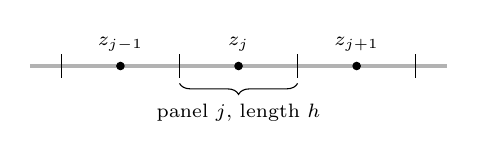
\begin{tikzpicture}[x=1cm,y=1cm,mdot/.style={circle,fill=black,inner sep=1.1pt}]
\draw[gray!60,line width=1.6pt] (-0.4,0) -- (4.9,0);
\foreach \x in {0,1.5,3,4.5} \draw (\x,0.15) -- (\x,-0.15);
\foreach \x/\l in {0.75/{j-1},2.25/j,3.75/{j+1}} {
  \node[mdot] at (\x,0) {};
  \node[font=\scriptsize,above=2pt] at (\x,0) {$z_{\l}$};}
\draw[decorate,decoration={brace,mirror,amplitude=4pt}] (1.5,-0.22) -- (3,-0.22)
  node[midway,below=4pt,font=\scriptsize] {panel $j$, length $h$};
\end{tikzpicture}}

% \junctionzoom: one junction, not to scale. Panels (thin ticks, small dots), chunks of p = 4
% panels (thick ticks, coloured), the TQS node of each chunk (big dot) and the tree edges.
\colorlet{chA}{teal!70!black}
\colorlet{chB}{red!70!black}
\colorlet{chC}{violet!80!black}
\colorlet{chL}{orange!85!black}
\colorlet{chR}{blue!70!black}
\newcommand{\junctionzoom}{%
\begin{tikzpicture}[x=1.85mm,y=1.85mm,
  mdot/.style={circle,fill=black,inner sep=0.5pt},
  ndot/.style={circle,fill=##1,inner sep=2pt}]
% chunks: name / colour / start / direction / label position
\foreach \c/\col/\sx/\sy/\dx/\dy in {A/chA/0/-8/0/1, B/chB/0/-4/0/1, C/chC/0/0/0/1, L/chL/0/0/-1/0, R/chR/0/0/1/0} {
  \draw[\col,line width=2pt,opacity=0.35] (\sx,\sy) -- ++(4*\dx,4*\dy);
  \foreach \k in {0,...,3} \node[mdot] at ($(\sx,\sy)+(\k*\dx+0.5*\dx,\k*\dy+0.5*\dy)$) {};
  \foreach \k in {1,2,3} \draw ($(\sx,\sy)+(\k*\dx,\k*\dy)+(0.3*\dy,0.3*\dx)$) -- ++(-0.6*\dy,-0.6*\dx);
  \draw[line width=0.9pt] ($(\sx,\sy)+(0.8*\dy,0.8*\dx)$) -- ++(-1.6*\dy,-1.6*\dx);
  \draw[line width=0.9pt] ($(\sx,\sy)+(4*\dx,4*\dy)+(0.8*\dy,0.8*\dx)$) -- ++(-1.6*\dy,-1.6*\dx);
}
\draw[dotted,thick] (0,-8) -- ++(0,-1.5) (0,4) -- ++(0,1.5) (-4,0) -- ++(-1.5,0) (4,0) -- ++(1.5,0);
\node[circle,draw,fill=white,inner sep=1.3pt] at (0,0) {};
\draw[->,gray] (-3.2,-3.2) node[below left=-2pt,font=\tiny,text=black,align=center] {junction\\(no unknown)} -- (-0.35,-0.35);
\foreach \c/\col/\lx/\ly in {A/chA/1.6/-6, B/chB/1.6/-2.6, C/chC/1.6/2.5, L/chL/-2.5/1.3, R/chR/3/-1.3}
  \node[font=\scriptsize,text=\col] at (\lx,\ly) {$\c$};
% the tree drawn to the right
\begin{scope}[shift={(15,-2)}]
\node[ndot=chA] (A) at (0,-5) {}; \node[ndot=chB] (B) at (0,-1) {};
\node[ndot=chC] (C) at (0,3) {}; \node[ndot=chL] (L) at (-3.5,2) {}; \node[ndot=chR] (R) at (3.5,2) {};
\draw[thick] (A) -- (B) (B) -- (C) (B) -- (L) (B) -- (R);
\foreach \c/\pos in {A/right,B/right,C/right,L/above,R/above} \node[font=\scriptsize,\pos=2pt] at (\c) {$\c$};
\draw[dotted,thick] (A) -- ++(0,-2) (C) -- ++(0,2) (L) -- ++(-2,0) (R) -- ++(2,0);
\end{scope}
\end{tikzpicture}}

% \antennawave{scale}: the antenna (no discretization) hit by a plane wave u^inc in direction d,
% with outgoing scattered wavefronts u^s
\newcommand{\antennawave}[1]{%
\begin{tikzpicture}[x=#1,y=#1]
\draw[line width=1.6pt] (0,0) -- (0,3.5) (-1.5,1) -- (1.5,1) (-1,2) -- (1,2) (-0.5,3) -- (0.5,3);
\foreach \t in {0,0.35,0.7}
  \draw[teal!70!black,thick] ($(-2.3,3.9)+\t*(0.8,-0.6)+(-0.54,-0.72)$) -- ($(-2.3,3.9)+\t*(0.8,-0.6)+(0.54,0.72)$);
\draw[->,teal!70!black,thick] (-2.0,3.0) -- ++($0.7*(0.8,-0.6)$) node[below,font=\scriptsize] {$d$};
\node[teal!70!black,font=\scriptsize,above] at (-1.9,4.65) {$u^{\mathrm{inc}}=e^{ik\,d\cdot x}$};
\foreach \r in {2.3,2.65,3.0}
  \draw[orange!80!black,thick,dashed] ($(0,1.75)+(-50:\r)$) arc (-50:35:\r);
\node[orange!80!black,font=\scriptsize,right] at ($(0,1.75)+(10:3.0)$) {$u^{s}$};
\node[font=\scriptsize] at (-0.95,0.35) {$\Gamma$};
\node[font=\scriptsize] at (-1.9,0.2) {$\mathbb{R}^2\setminus\Gamma$};
\end{tikzpicture}}

\title{Solving an integral equation with TQS:\\ an antenna model problem}
\date{}

% section divider slide at the start of every section
\AtBeginSection[]{%
\begin{frame}[plain,noframenumbering]
\centering\vfill
{\usebeamercolor[fg]{frametitle}\Large\insertsection\par}
\vfill
\end{frame}}

\begin{document}

\begin{frame}
\titlepage
\end{frame}

\section{From the Helmholtz problem to an integral equation}

% --------------------------------------------------------------------------
\begin{frame}{Exterior Helmholtz problem in 2D}
\begin{columns}[c]
\begin{column}{0.45\textwidth}
\centering
\antennawave{1.05cm}
\end{column}
\begin{column}{0.54\textwidth}
\small
$\Gamma$: union of open arcs (line segments), $x\in\mathbb{R}^2\cong\mathbb{C}$.

\vspace{1mm}
Given $u^{\mathrm{inc}}$, find the scattered field $u^s$:
\begin{align*}
\Delta u^s+k^2u^s&=0 && \text{in } \mathbb{R}^2\setminus\Gamma,\\
u^s&=-u^{\mathrm{inc}} && \text{on } \Gamma,\\
\sqrt{r}\,\big(\partial_r u^s-ik\,u^s\big)&\to0 && r=|x|\to\infty.
\end{align*}
\begin{itemize}
\item $k>0$: wavenumber; $d$: unit direction of $u^{\mathrm{inc}}$
\item Boundary condition: total field $u^{\mathrm{inc}}+u^s$ vanishes on $\Gamma$
\item Radiation condition: $u^s$ is outgoing
\end{itemize}
\end{column}
\end{columns}
\end{frame}

% --------------------------------------------------------------------------
\begin{frame}{Boundary integral formulation}
\small
Outgoing fundamental solution: $G_k(x,y)=\tfrac{i}{4}H_0^{(1)}(k|x-y|)$, \ $(\Delta+k^2)\,G_k(\cdot,y)=-\delta_y$
\quad ($H_0^{(1)}$: Hankel function).

\vspace{2mm}
\textbf{Ansatz} (single-layer potential) with an unknown density $\sigma$ on $\Gamma$:
\[
u^s(x)=\int_\Gamma G_k(x,w)\,\sigma(w)\,|dw|,\qquad x\in\mathbb{R}^2\setminus\Gamma.
\]
\begin{itemize}
\item Satisfies the Helmholtz equation and the radiation condition automatically
\item Continuous across $\Gamma$; $\sigma$ $=$ jump of $\partial_n u^s$ across $\Gamma$
\end{itemize}
\textbf{Boundary condition} $u^s=-u^{\mathrm{inc}}$ on $\Gamma$ gives a \emph{first-kind} equation:
\[
\int_\Gamma G_k(z,w)\,\sigma(w)\,|dw|=-u^{\mathrm{inc}}(z),\qquad z\in\Gamma.
\]
\begin{itemize}
\item Unknown only on $\Gamma$: 2D problem $\to$ 1D equation on the tree of segments
\item Kernel log-singular: $G_k(z,w)\sim-\tfrac{1}{2\pi}\log|z-w|$; dense matrix after discretization
\end{itemize}
\end{frame}

\section{Testing TQS on a model problem}

% --------------------------------------------------------------------------
\begin{frame}{A model problem with a simpler kernel}
\begin{columns}[c]
\begin{column}{0.42\textwidth}
\centering
\antennaplain{1.45cm}
\end{column}
\begin{column}{0.57\textwidth}
\small
Keep $\Gamma$ (total length $9.5$) and the first-kind equation; simplify the kernel:
\[
\underbrace{\int_\Gamma |z-w|^\alpha\,u(w)\,|dw|}_{(\mathcal K u)(z)} = f(z),\qquad z\in\Gamma.
\]
\begin{itemize}
\item $G_k\to|z-w|^\alpha$, $0<\alpha<1$: real, not oscillatory, not smooth at $z=w$
  \ (note $(|z-w|^\alpha-1)/\alpha\to\log|z-w|$ as $\alpha\to0$)
\item $u\leftrightarrow\sigma$, \ $f\leftrightarrow-u^{\mathrm{inc}}$
\item Here: $\alpha=\tfrac12$, $f\equiv1$
\end{itemize}
\end{column}
\end{columns}
\end{frame}

% --------------------------------------------------------------------------
\begin{frame}{Discretization: panels and midpoints}
\begin{columns}[c]
\begin{column}{0.42\textwidth}
\centering
\antennapanels{1.45cm}

\vspace{1mm}
{\scriptsize $P=4$ shown; experiments: $P=32,64,128$}
\end{column}
\begin{column}{0.57\textwidth}
\small
\begin{itemize}
\item Panels of length $h=1/P$; $N=9.5\,P$ panels
\item Midpoints $z_j$; unknowns $u_j\approx u(z_j)$
\end{itemize}
\vspace{1mm}
\centering
\panelzoom
\vspace{1mm}
\raggedright
\begin{itemize}
\item Collocate at $z_i$, midpoint rule:
\[
(\mathcal K u)(z_i)\approx\sum_{j} \mathrm{K}_{ij}\,u_j,\quad \mathrm{K}_{ij}\approx h\,|z_i-z_j|^\alpha
\]
\item Junctions are panel ends: no unknown there
\end{itemize}
\end{column}
\end{columns}
\end{frame}

% --------------------------------------------------------------------------
\begin{frame}{Discretization: the linear system}
\small
$N$ equations for $u_1,\dots,u_N$:
\[
\sum_{j=1}^N \mathrm{K}_{ij}\,u_j=f(z_i),\qquad
\mathrm{K}_{ij}=\begin{cases}
h\,|z_i-z_j|^\alpha, & i\neq j \quad\text{(midpoint rule)},\\[2pt]
\displaystyle\int_{-h/2}^{h/2}|t|^\alpha\,dt=\frac{2\,(h/2)^{1+\alpha}}{1+\alpha}, & i=j \quad\text{(exact)}.
\end{cases}
\]
$\mathrm{K}u=f$: dense, $N\times N$, real symmetric.
\end{frame}

% --------------------------------------------------------------------------
\begin{frame}{Spectrum of $\mathrm{K}$}
\begin{columns}[c]
\begin{column}{0.6\textwidth}
\centering
\begin{tikzpicture}
\begin{axis}[
  width=\textwidth, height=0.5\textheight,
  xlabel={eigenvalues $\mu_k$ of $\mathrm{K}$}, title={\footnotesize one eigenvalue ($\approx10.3$) off scale},
  xmin=-2.5, xmax=0.3, ymin=0.4, ymax=3.6,
  ytick={1,2,3}, yticklabels={$N=1216$,$N=608$,$N=304$},
  tick label style={font=\scriptsize}, label style={font=\footnotesize},
  grid=major, grid style={gray!20}]
\draw[sub, thick] (axis cs:0,0.4) -- (axis cs:0,3.6);
\addplot[only marks, mark=|, mark size=4pt, rest, restrict x to domain=-3:1] table[x=mu, y expr=3] {spectrum_304.dat};
\addplot[only marks, mark=|, mark size=4pt, rest, restrict x to domain=-3:1] table[x=mu, y expr=2] {spectrum_608.dat};
\addplot[only marks, mark=|, mark size=4pt, rest, restrict x to domain=-3:1] table[x=mu, y expr=1] {spectrum_1216.dat};
\end{axis}
\end{tikzpicture}
\end{column}
\begin{column}{0.38\textwidth}
\centering\small
\begin{tabular}{@{}rcc@{}}
\toprule
$N$ & $\min_k|\mu_k|$ & $\operatorname{cond}(\mathrm{K})$ \\
\midrule
304  & $1.0\cdot10^{-3}$ & $9.9\cdot10^{3}$ \\
608  & $3.7\cdot10^{-4}$ & $2.8\cdot10^{4}$ \\
1216 & $1.3\cdot10^{-4}$ & $7.9\cdot10^{4}$ \\
\bottomrule
\end{tabular}
\end{column}
\end{columns}

\vspace{2mm}
\small
\begin{itemize}
\item One positive eigenvalue; the other $N-1$ in $[-2.29,0)$, accumulating at $0$
\item First kind: $\operatorname{cond}(\mathrm{K})\sim N^{1+\alpha}$ (unbounded inverse)
\item Indefinite $\Rightarrow$ GMRES
\end{itemize}
\end{frame}

% --------------------------------------------------------------------------
\begin{frame}{TQS approximation of $\mathrm{K}$}
\begin{columns}[c]
\begin{column}{0.40\textwidth}
\centering
\antenna{1.3cm}{1}
\end{column}
\begin{column}{0.59\textwidth}
\centering
\junctionzoom

{\scriptsize junction zoom, $p=4$ shown}

\vspace{1mm}
\raggedright\footnotesize
\begin{enumerate}
\item \textbf{Chunking:} $p$ consecutive panels $\to$ one node ($p=8$); node $=$ $p$ unknowns
\item \textbf{Graph:} edges between neighbouring chunks; junction hub $B$ $\to$ $C,L,R$.
  \texttt{GraphPartitionedMatrix}: $\mathrm{K}$ with one $p\times p$ block per node pair
\item \textbf{Tree $\to$ TQS:} root at the base. \texttt{TQSMatrix}$(\cdot,1,\varepsilon,\infty)$ compresses each Hankel block
  $\mathrm{K}(\textcolor{rest}{\overline{S(k)}},\textcolor{sub}{S(k)})$ by truncated SVD at tolerance $\varepsilon$; its rank is $\rho_{k,\mathcal P(k)}$
\end{enumerate}
{\scriptsize $S(k)$: subtree of $k$; $\mathcal P(k)$: parent of $k$}
\end{column}
\end{columns}
\end{frame}

% --------------------------------------------------------------------------
\begin{frame}{Compression of $\mathrm{K}$ by TQS}
\small
$p=8$. memory $=$ floats in all generators ($\mathrm{D}$, \texttt{inp}, \texttt{out}, \texttt{trans}) $/\,N^2$.
\vspace{1mm}
\begin{columns}[T]
\begin{column}{0.6\textwidth}
\centering
Fixed $N=4864$ ($608$ nodes), varying $\varepsilon$\\[1mm]
\footnotesize
\begin{tabular}{@{}rrrcc@{}}
\toprule
$\varepsilon$ & $\max\rho$ & mean $\rho$ & $\frac{\|\mathrm{K}-\mathrm{T}_\varepsilon\|_F}{\|\mathrm{K}\|_F}$ & memory \\
\midrule
$10^{-1}$  & 1  & 1.0  & $1.0\cdot10^{-1}$  & 0.25\,\% \\
$10^{-2}$  & 3  & 1.9  & $3.2\cdot10^{-2}$  & 0.34\,\% \\
$10^{-4}$  & 10 & 4.8  & $5.8\cdot10^{-4}$  & 0.69\,\% \\
$10^{-6}$  & 19 & 8.8  & $6.6\cdot10^{-6}$  & 1.36\,\% \\
$10^{-8}$  & 29 & 13.0 & $6.6\cdot10^{-8}$  & 2.26\,\% \\
$10^{-10}$ & 38 & 17.1 & $6.8\cdot10^{-10}$ & 3.33\,\% \\
$10^{-12}$ & 47 & 21.1 & $6.7\cdot10^{-12}$ & 4.62\,\% \\
\bottomrule
\end{tabular}
\end{column}
\begin{column}{0.36\textwidth}
\centering
Fixed $\varepsilon=10^{-8}$, varying $N$\\[1mm]
\footnotesize
\begin{tabular}{@{}rrrr@{}}
\toprule
$N$ & nodes & $\max\rho$ & mean $\rho$ \\
\midrule
304  & 38  & 24 & 11.5 \\
608  & 76  & 26 & 11.9 \\
1216 & 152 & 27 & 12.3 \\
2432 & 304 & 28 & 12.7 \\
4864 & 608 & 29 & 13.0 \\
\bottomrule
\end{tabular}
\end{column}
\end{columns}
\vspace{2mm}
\begin{itemize}
\item $\max\rho$ grows by $\approx4.6$ per decade of $\varepsilon$ and by $\approx1$ per doubling of $N$
\item ULV solve: $O\big(\#\text{nodes}\cdot(p+\max\rho)^3\big)$, nearly linear in $N$
\end{itemize}
\end{frame}

% --------------------------------------------------------------------------
\begin{frame}{The algorithm}
\small
\begin{algorithm}[H]
\caption{TQS-preconditioned Krylov solve}
\begin{algorithmic}[1]
\State Build panels, midpoints and tree
\State Build the TQS approximation $\mathrm{T}_\varepsilon\approx\mathrm{K}$ at tolerance $\varepsilon$
\State Preconditioner $\mathrm{M}:=\mathrm{T}_\varepsilon$; apply $\mathrm{M}^{-1}v$ by a ULV solve
\State GMRES on $\mathrm{K}\mathrm{M}^{-1}y=f$, then $x=\mathrm{M}^{-1}y$
\Statex \hspace{\algorithmicindent}each mat-vec $\mathrm{K}v$ by a fast multiply exploiting the kernel structure
\end{algorithmic}
\end{algorithm}
\begin{itemize}
\item $\varepsilon$: SVD truncation tolerance; $\max\rho$: largest state dimension
\item its: iterations to $\|f-\mathrm{K}x\|\le10^{-10}\|f\|$
\item Baseline: no preconditioner
\item \textbf{In these tests only:} $\mathrm{T}_\varepsilon$ is built from the dense $\mathrm{K}$ ($O(N^2)$) and $\mathrm{K}v$ is a dense mat-vec. In practice neither $\mathrm{K}$ nor its dense mat-vec is formed.
\end{itemize}
\end{frame}

% --------------------------------------------------------------------------
\begin{frame}{GMRES: compression error and iterations}
\small
$\operatorname{cond}(\mathrm{K})$: $9.9\cdot10^{3}$, $2.8\cdot10^{4}$, $7.9\cdot10^{4}$.\\[1mm]
its: number of GMRES iterations $k$ until the relative residual satisfies
\[
\frac{\|f-\mathrm{K}x_k\|_2}{\|f\|_2}\le10^{-10},\qquad x_0=0,\ \text{no restarts}.
\]
\vspace{-2mm}
\begin{center}
\begin{tabular}{@{}lccccccc@{}}
\toprule
& & \multicolumn{2}{c}{$N=304$} & \multicolumn{2}{c}{$N=608$} & \multicolumn{2}{c}{$N=1216$} \\
\cmidrule(lr){3-4}\cmidrule(lr){5-6}\cmidrule(l){7-8}
preconditioner & $\max\rho$ & $\frac{\|\mathrm{K}-\mathrm{T}_\varepsilon\|_2}{\|\mathrm{K}\|_2}$ & its & $\frac{\|\mathrm{K}-\mathrm{T}_\varepsilon\|_2}{\|\mathrm{K}\|_2}$ & its & $\frac{\|\mathrm{K}-\mathrm{T}_\varepsilon\|_2}{\|\mathrm{K}\|_2}$ & its \\
\midrule
none & -- & -- & 59 & -- & 78 & -- & 104 \\
TQS, $\varepsilon=10^{-1}$ & 1 & $5.5\cdot10^{-2}$ & 41 & $5.8\cdot10^{-2}$ & 54 & $6.0\cdot10^{-2}$ & 70 \\
TQS, $\varepsilon=10^{-2}$ & 3 & $7.2\cdot10^{-3}$ & 20 & $7.5\cdot10^{-3}$ & 27 & $7.8\cdot10^{-3}$ & 36 \\
TQS, $\varepsilon=10^{-4}$ & 10 & $6.6\cdot10^{-5}$ & 6 & $7.7\cdot10^{-5}$ & 7 & $1.0\cdot10^{-4}$ & 9 \\
TQS, $\varepsilon=10^{-8}$ & 24--27 & $7.6\cdot10^{-9}$ & 2 & $5.1\cdot10^{-9}$ & 2 & $8.0\cdot10^{-9}$ & 2 \\
\bottomrule
\end{tabular}
\end{center}
\end{frame}

% --------------------------------------------------------------------------
\begin{frame}{Convergence history ($N=1216$)}
\centering
\begin{tikzpicture}
\begin{semilogyaxis}[
  width=0.82\textwidth, height=0.62\textheight,
  xlabel={GMRES iteration}, ylabel={$\|f-\mathrm{K}x_k\|/\|f\|$},
  ymin=1e-11, ymax=2, xmin=0, xmax=110,
  legend pos=north east, legend style={font=\scriptsize}, legend cell align=left,
  unbounded coords=jump, grid=major, grid style={gray!20}]
\addplot[black, thick] table[x=it,y=none] {gmres_history.dat};
\addplot[orange!80!black, thick] table[x=it,y=tqs1e-02] {gmres_history.dat};
\addplot[rest, thick] table[x=it,y=tqs1e-04] {gmres_history.dat};
\addplot[sub, thick, mark=*, mark size=1pt] table[x=it,y=tqs1e-08] {gmres_history.dat};
\legend{none, {TQS $\varepsilon=10^{-2}$ ($\max\rho=3$)}, {TQS $\varepsilon=10^{-4}$ ($\max\rho=10$)}, {TQS $\varepsilon=10^{-8}$ ($\max\rho=27$)}}
\end{semilogyaxis}
\end{tikzpicture}
\end{frame}

\section{The Helmholtz problem: Galerkin BEM}

% --------------------------------------------------------------------------
\begin{frame}{Galerkin discretization of the single-layer equation}
\small
Same panels $\Gamma_1,\dots,\Gamma_N$ (length $h=1/P$, $N=9.5\,P$), same chunks ($p=8$) and same TQS tree.

\vspace{1mm}
Piecewise constant density $\sigma=\sum_j \sigma_j\,\varphi_j$, \ $\varphi_j$: indicator function of $\Gamma_j$; test with $\varphi_i$:
\[
\mathrm{V}\sigma=b,\qquad
\mathrm{V}_{ij}=\int_{\Gamma_i}\!\int_{\Gamma_j} G_k(x,y)\,|dy|\,|dx|,\qquad
b_i=-\int_{\Gamma_i}u^{\mathrm{inc}}(x)\,|dx|.
\]
\begin{itemize}
\item $\mathrm{V}$: dense, $N\times N$, complex symmetric ($\mathrm{V}^{\mathsf T}=\mathrm{V}$, not Hermitian)
\item Quadrature: self and touching panels: $G_k=-\tfrac{1}{2\pi}\log|x-y|+R_k(|x-y|)$ with $R_k$ smooth;
  the log part is integrated exactly over $\Gamma_j$, the rest by $8$-point Gauss. Other panels: tensor Gauss
  ($8\times8$ if near, $3\times3$ if the midpoints are $\ge4h$ apart). Entries accurate to $\approx10^{-5}$
\item $u^{\mathrm{inc}}(x)=e^{ik\,d\cdot x}$, \ $d=(0.8,-0.6)$
\item Check: $u^s(2.5+0.5i)$ changes by $\le10^{-3}$ when $N$ doubles
\end{itemize}
\end{frame}

% --------------------------------------------------------------------------
% \fieldplot{k}{title}: |u^inc + u^s| on a grid, antenna drawn on top
\newcommand{\fieldplot}[2]{%
\begin{tikzpicture}
\begin{axis}[
  width=0.98\textwidth, axis equal image, enlargelimits=false,
  xmin=-2.5, xmax=2.5, ymin=-0.75, ymax=4.25,
  title={\footnotesize #2}, tick label style={font=\tiny},
  colormap={vir}{rgb255=(68,1,84) rgb255=(59,82,139) rgb255=(33,145,140) rgb255=(94,201,98) rgb255=(253,231,37)},
  point meta min=0, point meta max=2.5,
  colorbar, colorbar style={width=2mm, tick label style={font=\tiny}}]
\addplot graphics[xmin=-2.5, xmax=2.5, ymin=-0.75, ymax=4.25] {helmholtz_field_k#1.png};
\draw[white, line width=0.6pt] (axis cs:0,0) -- (axis cs:0,3.5) (axis cs:-1.5,1) -- (axis cs:1.5,1)
  (axis cs:-1,2) -- (axis cs:1,2) (axis cs:-0.5,3) -- (axis cs:0.5,3);
\end{axis}
\end{tikzpicture}}

\begin{frame}{Two test cases: large and small wavelength}
\small
Wavelength $\lambda=2\pi/k$; plots: total field $|u^{\mathrm{inc}}+u^s|$, $N=1216$.
\begin{columns}[T]
\begin{column}{0.49\textwidth}
\centering
\fieldplot{1}{$k=1$: $\lambda\approx6.3$ (easy)}

\vspace{-1mm}
\scriptsize $\lambda$ larger than $\Gamma$; $400$--$1600$ panels per $\lambda$
\end{column}
\begin{column}{0.49\textwidth}
\centering
\fieldplot{40}{$k=40$: $\lambda\approx0.16$}

\vspace{-1mm}
\scriptsize $\Gamma$ (length $9.5$) is $\approx60\lambda$ long; $10$--$40$ panels per $\lambda$
\end{column}
\end{columns}
\end{frame}

% --------------------------------------------------------------------------
\begin{frame}{The algorithm for Helmholtz}
\small
\begin{algorithm}[H]
\caption{TQS-preconditioned GMRES for $\mathrm{V}\sigma=b$}
\begin{algorithmic}[1]
\State Build panels, chunks and tree (as before)
\State Build the TQS approximation $\mathrm{T}_\varepsilon\approx\mathrm{V}$ (complex) at tolerance $\varepsilon$
\State Preconditioner $\mathrm{M}:=\mathrm{T}_\varepsilon$; apply $\mathrm{M}^{-1}v$ by a ULV solve
\State GMRES on $\mathrm{V}\mathrm{M}^{-1}y=b$, then $\sigma=\mathrm{M}^{-1}y$
\Statex \hspace{\algorithmicindent}each mat-vec $\mathrm{V}v$ by a fast multiply
\end{algorithmic}
\end{algorithm}
\vspace{-1mm}
\begin{block}{Mat-vec}
\begin{itemize}
\item Should be an FMM for $G_k$ ($O(N)$ for small $k$; a high-frequency / directional FMM for large $k$), with near-field corrections from the BEM quadrature
\item \textbf{For now:} dense $\mathrm{V}v$, and $\mathrm{T}_\varepsilon$ built from the dense $\mathrm{V}$. This already tests the framework: the iteration counts do not depend on how $\mathrm{V}v$ is computed (up to the FMM accuracy)
\end{itemize}
\end{block}
its: GMRES iterations until $\|b-\mathrm{V}\sigma_k\|_2\le10^{-10}\|b\|_2$ ($\sigma_0=0$, no restarts).
\end{frame}

% --------------------------------------------------------------------------
\begin{frame}{Compression of $\mathrm{V}$ by TQS}
\small
$N=2432$ ($304$ nodes), $p=8$. memory $=$ floats in all generators $/\,N^2$.
\vspace{2mm}
\begin{center}
\begin{tabular}{@{}rcccccccc@{}}
\toprule
& \multicolumn{4}{c}{$k=1$} & \multicolumn{4}{c}{$k=40$} \\
\cmidrule(lr){2-5}\cmidrule(l){6-9}
$\varepsilon$ & $\max\rho$ & mean $\rho$ & $\frac{\|\mathrm{V}-\mathrm{T}_\varepsilon\|_F}{\|\mathrm{V}\|_F}$ & memory
              & $\max\rho$ & mean $\rho$ & $\frac{\|\mathrm{V}-\mathrm{T}_\varepsilon\|_F}{\|\mathrm{V}\|_F}$ & memory \\
\midrule
$10^{-2}$  & 4  & 2.7  & $2.7\cdot10^{-2}$  & 0.9\,\% & 28 & 10.3 & $1.7\cdot10^{-2}$  & 3.6\,\% \\
$10^{-4}$  & 13 & 6.7  & $3.2\cdot10^{-4}$  & 2.0\,\% & 36 & 14.8 & $1.7\cdot10^{-4}$  & 5.8\,\% \\
$10^{-6}$  & 21 & 10.5 & $3.1\cdot10^{-6}$  & 3.4\,\% & 44 & 18.7 & $1.7\cdot10^{-6}$  & 8.1\,\% \\
$10^{-8}$  & 29 & 14.2 & $3.2\cdot10^{-8}$  & 5.1\,\% & 51 & 22.5 & $1.7\cdot10^{-8}$  & 10.6\,\% \\
$10^{-10}$ & 37 & 17.9 & $3.0\cdot10^{-10}$ & 7.2\,\% & 58 & 25.9 & $1.6\cdot10^{-10}$ & 13.3\,\% \\
\bottomrule
\end{tabular}
\end{center}
\begin{itemize}
\item $k=1$: like the model problem ($\max\rho$ grows by $\approx4$ per decade of $\varepsilon$)
\item $k=40$: $\max\rho$ larger by $\approx21$--$24$ (oscillations); growth per decade of $\varepsilon$ about the same
\item Memory: complex entries, counted as for the model problem
\end{itemize}
\end{frame}

% --------------------------------------------------------------------------
\begin{frame}{GMRES iterations}
\small
\begin{center}
\begin{tabular}{@{}rrrrrccc@{}}
\toprule
& & & & & \multicolumn{3}{c}{TQS: its ($\max\rho$)} \\
\cmidrule(l){6-8}
$k$ & $N$ & panels/$\lambda$ & $\operatorname{cond}(\mathrm{V})$ & none & $\varepsilon=10^{-2}$ & $\varepsilon=10^{-4}$ & $\varepsilon=10^{-8}$ \\
\midrule
1  & 608  & 402  & $8.5\cdot10^{2}$ & 64  & 13 (4)  & 4 (12) & 2 (26) \\
1  & 1216 & 804  & $1.7\cdot10^{3}$ & 79  & 16 (4)  & 4 (13) & 2 (27) \\
1  & 2432 & 1608 & $3.4\cdot10^{3}$ & 97  & 20 (4)  & 5 (13) & 2 (29) \\
\midrule
40 & 608  & 10   & $5.9\cdot10^{1}$ & 111 & 7 (28)  & 3 (35) & 2 (47) \\
40 & 1216 & 20   & $1.2\cdot10^{2}$ & 133 & 9 (28)  & 3 (35) & 2 (49) \\
40 & 2432 & 40   & $2.5\cdot10^{2}$ & 159 & 11 (28) & 4 (36) & 2 (51) \\
\bottomrule
\end{tabular}
\end{center}
\begin{itemize}
\item $\operatorname{cond}(\mathrm{V})\sim N$ (first kind); without preconditioner the iterations grow with $N$ and with $k$
\item TQS, $\varepsilon=10^{-4}$: $3$--$5$ iterations for both wavelengths
\item $\|\mathrm{V}-\mathrm{T}_\varepsilon\|_2/\|\mathrm{V}\|_2\approx\varepsilon$ in all cases
\end{itemize}
\end{frame}

% --------------------------------------------------------------------------
\begin{frame}{Convergence history ($N=1216$, TQS $\varepsilon=10^{-4}$)}
\centering
\begin{tikzpicture}
\begin{semilogyaxis}[
  width=0.82\textwidth, height=0.62\textheight,
  xlabel={GMRES iteration}, ylabel={$\|b-\mathrm{V}\sigma_k\|/\|b\|$},
  ymin=1e-11, ymax=2, xmin=0, xmax=140,
  legend pos=north east, legend style={font=\scriptsize}, legend cell align=left,
  unbounded coords=jump, grid=major, grid style={gray!20}]
\addplot[rest, thick, dashed] table[x=it,y=none_k1] {helmholtz_gmres_history.dat};
\addplot[sub, thick, dashed] table[x=it,y=none_k40] {helmholtz_gmres_history.dat};
\addplot[rest, thick, mark=*, mark size=1pt] table[x=it,y=tqs_k1] {helmholtz_gmres_history.dat};
\addplot[sub, thick, mark=*, mark size=1pt] table[x=it,y=tqs_k40] {helmholtz_gmres_history.dat};
\legend{{$k=1$, none}, {$k=40$, none}, {$k=1$, TQS ($\max\rho=13$)}, {$k=40$, TQS ($\max\rho=35$)}}
\end{semilogyaxis}
\end{tikzpicture}
\end{frame}

% --------------------------------------------------------------------------
\begin{frame}{Takeaways and next steps}
\small
\textbf{Takeaways}
\begin{itemize}
\item The antenna is a natural TQS tree; $\max\rho$ grows like $\log N$
\item Model problem: TQS preconditioner ($\varepsilon=10^{-4}$, $\max\rho=10$): $104\to9$ GMRES iterations at $N=1216$
\item Helmholtz, Galerkin BEM: TQS preconditioner ($\varepsilon=10^{-4}$): $\le5$ iterations for $k=1$ and $k=40$;
  small wavelength costs larger ranks ($\max\rho\approx36$ vs.\ $13$), not more iterations
\end{itemize}
\textbf{Next steps}
\begin{enumerate}
\item FMM mat-vec for $\mathrm{V}$ in the Krylov loop; wall-clock times
\item Build $\mathrm{T}_\varepsilon$ from the kernel (or from the FMM), without dense $\mathrm{K}$ or $\mathrm{V}$
\item Rank growth with $k$ at fixed panels per wavelength
\item Leaf-oriented tree; higher order quadrature
\end{enumerate}
\end{frame}

\end{document}
